L’analyse des résultats de tracking est essentielle pour évaluer la qualité de l’estimation de la trajectoire générée par notre système. Nous avons comparé les trajectoires issues de notre dispositif embarqué sur Raspberry Pi avec celles obtenues via des applications mobiles de référence utilisées simultanément sur nos téléphones.\\

Pour l'analyse nous allons prendre un exemple d'acquision.

La première image (Figure 1) montre la trajectoire enregistrée par notre systeme, affichée sur une carte OpenStreetMap. 
Le parcours suit globalement le trajet effectué à pied autour du campus de l’Université de Rouen, incluant des changements de direction, des passages étroits et des zones d’arrêt. 
Cependant nous remarquqons certains piques dans la trajectoire, cela traduit une estimation de trajectoire assez instable, nous voyons aussi un point completèment aberrant.

Nous pouvons aussi analyser la trajectoire enregistrée sur notre telephone lors d'une autre acquisiton.\\

La deuxieme image (Figure 2) nous montre la superposition des trajectoires de deux telephones. On voit que la trajectoire est un peu plus stable mais nous voyons aussi que, lors de l'entrée dans le bâtiment Magellan, les mesures sont bien moins précise, cela nous montre la limite de l'acquisiton GPS sur nos téléphones.

Cette différence s'explique par plusieurs facteurs :

\begin{itemize}
	\item Le GPS utilisé sur la Raspberry Pi est moins performant que les capteurs embarqués dans les téléphones modernes, notamment en ce qui concerne le taux de rafraîchissement et la sensibilité du module.
	\item Les erreurs d'intégration de l'IMU ou des problèmes de synchronisation entre les capteurs peuvent aussi induire des écarts cumulés.
\end{itemize}



Malgré cela, la trajectoire obtenue reste exploitable pour une première version du système. Elle reflète de manière satisfaisante la forme générale du parcours et permet une visualisation correcte de l’itinéraire parcouru. Des améliorations pourraient être envisagées, comme une fusion plus poussée des données ou l'ajout d’un système de correction GPS.



\begin{figure}[H] 
  \centering
  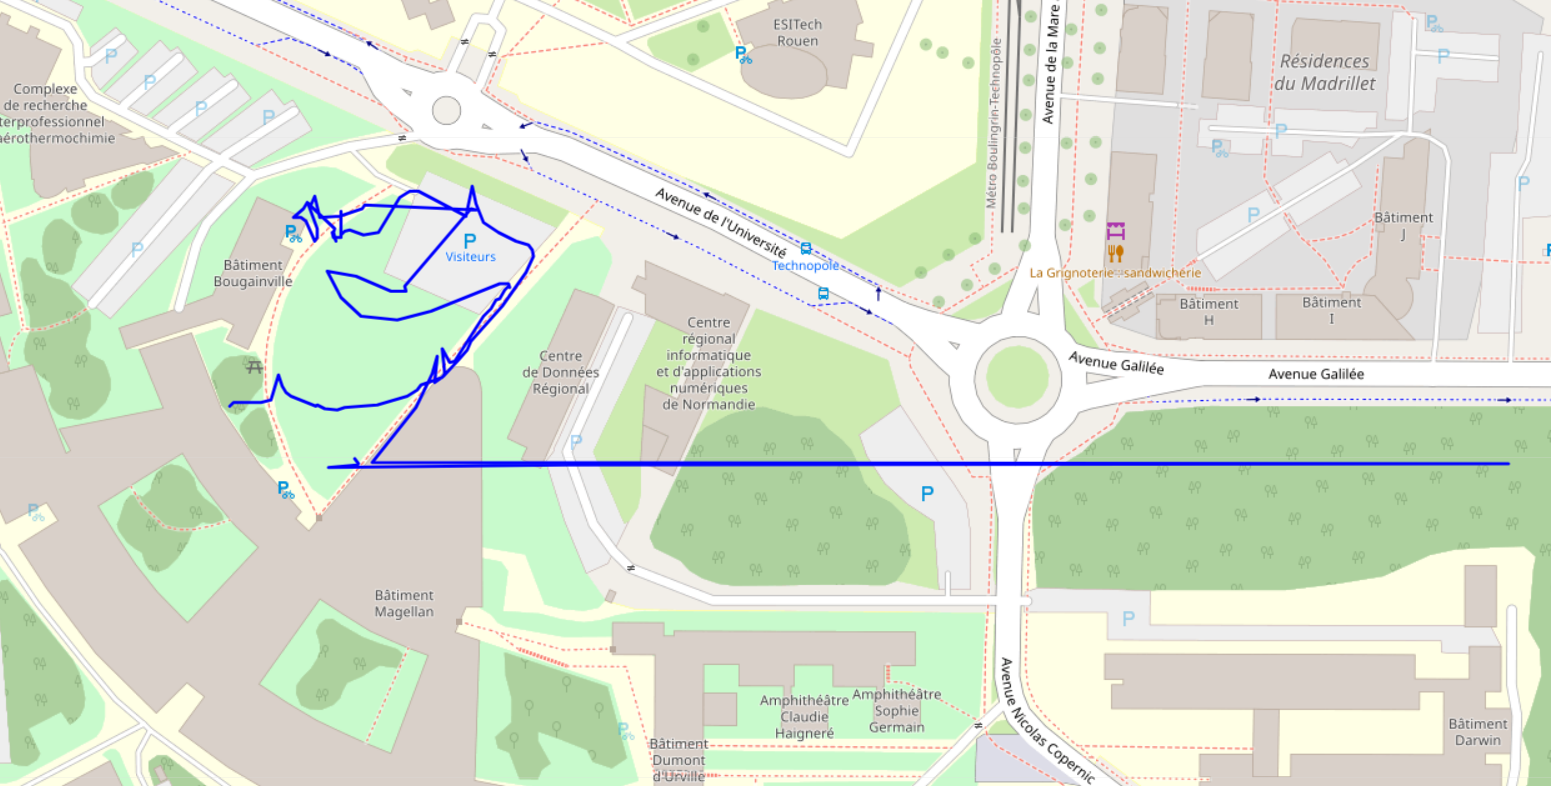
\includegraphics[width=0.7\textwidth]{OpenSM.png}
  \caption{Résultat système d'acquisiton sur OpenStreetMap}
\end{figure}

\begin{figure}[H] 
  \centering
  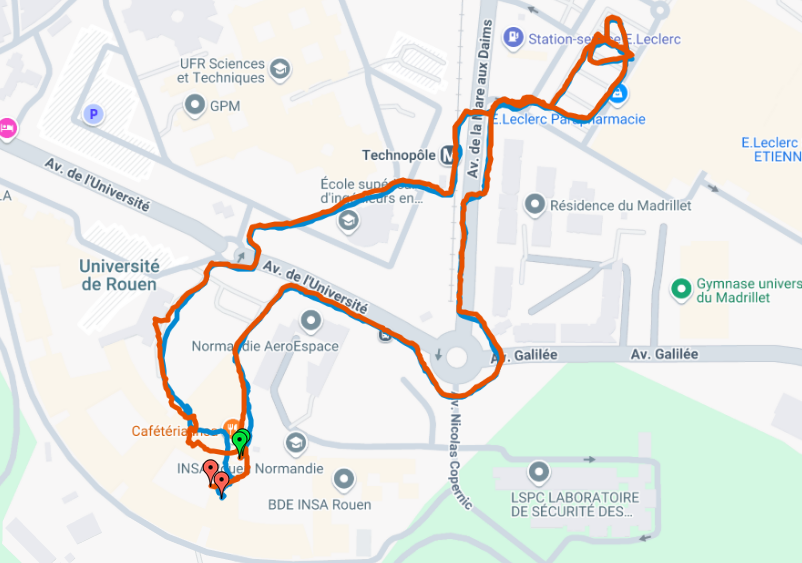
\includegraphics[width=0.7\textwidth]{superposition.png}
  \caption{Visualisation superposition trajectoire}
\end{figure}



